\documentclass[11pt]{article}

\title{{\Large Exact, Discrete, Multi-objective Optimization} \\ ECE498A Detailed Design Document}
\author{Joseph Hong, Chris Kleynhans, Ming-Ho Yee, Atulan Zaman \\
          Group 38}

% For definitions
\usepackage{amsthm}
\theoremstyle{definition}
\newtheorem{mydef}{Definition}

% TikZ is what lets us draw graphics
\usepackage{tikz}
\usetikzlibrary{shapes.multipart,positioning,arrows}

\usepackage{graphicx}
% For table
\usepackage{float}

%For table caption
\usepackage{caption}

%For limited depth table of content
\usepackage{titletoc}


%Declaring new column types for multiline columns
\usepackage{array}
\newcolumntype{L}[1]{>{\raggedright\let\newline\\\arraybackslash\hspace{0pt}}m{#1}}
\newcolumntype{C}[1]{>{\centering\let\newline\\\arraybackslash\hspace{0pt}}m{#1}}
\newcolumntype{R}[1]{>{\raggedleft\let\newline\\\arraybackslash\hspace{0pt}}m{#1}}

\begin{document}
\maketitle
\pagenumbering{roman}

\newpage
\tableofcontents
% Sets table of content of depth 1
\addtocontents{toc}{\setcounter{tocdepth}{1}}

\listoffigures

\newpage

\pagenumbering{arabic}

\section{High Level Design}\label{sec:high_level}
Multi-objective optimization is a widely researched area of computer
science that focuses on finding solutions to problem definitions with
respect to given objective realization constraints. Computing such
solutions is extremely resource intensive, and the computation time
grows exponentially with the number of optimization variables.

The nature of our work in scientific terms is called \textit{exact,
discrete multi-objective optimization}. Multi-objective optimization
(MOO) is the process of computing the most optimal solutions given a
goal and a set of constraints. The system we work on for our project is called Moolloy \cite{ref:Rayside09}.

The objective of our project is to optimize Moolloy's current algorithm of multi-objective optimization to make it run faster and with better memory efficiency. The current Moolloy uses an algorithm called Guided Improvement Algorithm which is a great multi-objective problem solver for problems with a limited metric scope, however for most real life problems and significant problems have higher number of objectives and higher number of metrices to solve for which are currently unsolvable by Moolloy due to an explosion of solution sets that are returned by the SAT solver for each metric point and also the fact that all of these solution need to be stored in memory in order to build on the constraints to find solutions. In our current testing architecture of 28 cores in the University of Waterloo CS laboratories, some of the models have ran for little more than 2 months before we had to shut down the computations.

The focus of this project is primarily to explore possible ideas to optimize the ``Guided Improvement Algorithm'' by researching existing optimization technniques for solver engines. As we have found out from our work on this project this is quite a difficult task because some of the the optimization ideas are quite complex to implement given the algorithm itself is very complex implementation. The details of the implementation challenges are discussed in more detail in the implementation section of the document.

The high-level design description contains two parts: \emph{Design Components} \& \emph{Testing Dashboard}. The first section is a description of the overall structure of our design and the components, and the second section is a description of the testing environment we created to help us along the design process.

\subsection{Design Components}

\begin{figure}
\caption{Major Components} \label{fig:components}
 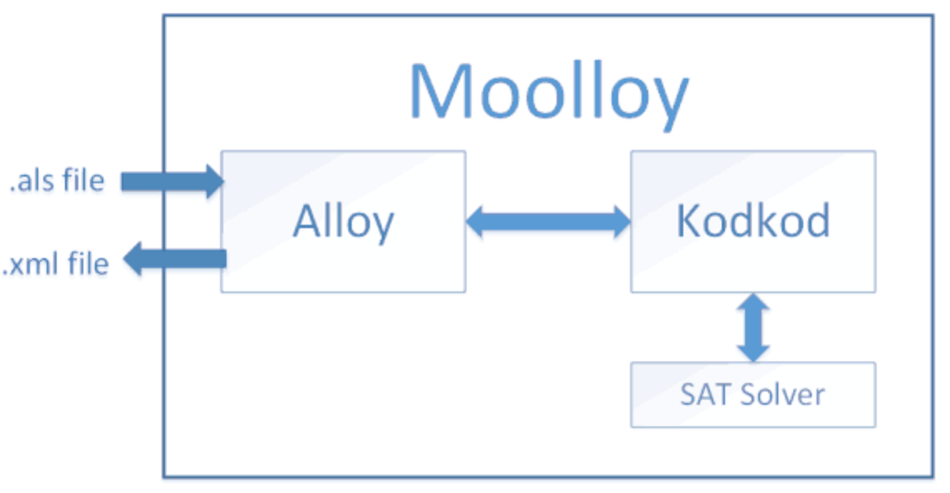
\includegraphics[width=\textwidth]{images/components}
\end{figure}

The design structure for Moolloy basically has three components: \emph{Alloy}, \emph{Kodkod}, and the \emph{SAT solver} that are interconnected to perform different functions starting from accepting the problem description written according to the Alloy relational modelling language and produce the results after the computations are finished in the form of a XML file. The overall structure for the Moolloy system is shown in Figure \ref{fig:components}. The detailed description of the function for each of the components are described in Section \ref{sec:components}.

\subsection{Testing Dashboard}
\begin{figure}
	\caption{Testing Dashboard} \label{fig:dashboard}
	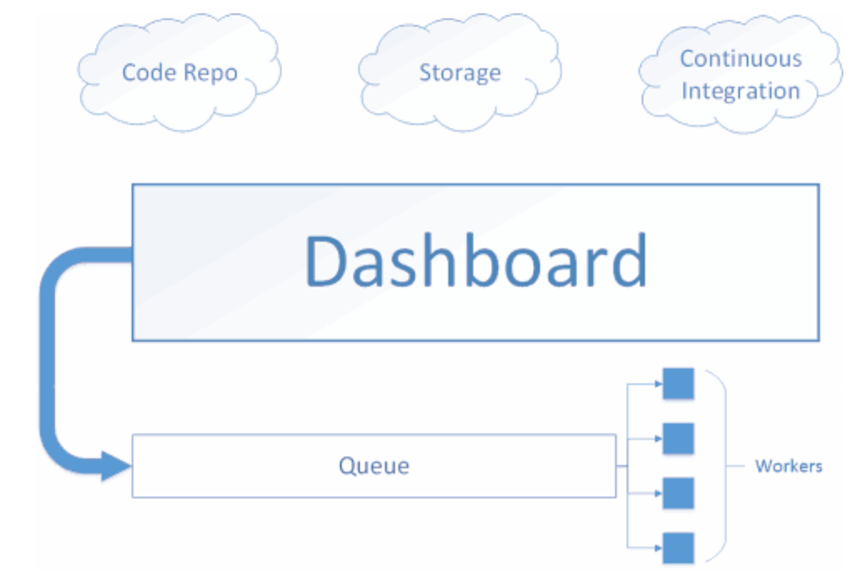
\includegraphics[width=\textwidth]{images/dashboard}
\end{figure}

Since this is a research project focused on optimization, one of the most important parts of our project is building a depedadable testing infrastructure and profiling system with which we can verify our work. Also, since we shall be working on a existing code base, and much of the computation in the system is done by an existing non-open source package, it is very important for us to build our development around a reliable environment with proper unit tests and continuous integration with the build system. Therefore, we spent much of our time creating a dependable and working testing infrastructure with a GUI dashboard which would make our development much more fluent going forward. The diagram for the testing dashboard structure is shown figure \ref{fig:dashboard}.

In this diagram we basically have two categories of components. The first category is a set of cloud services we are using for our project for different purposes which are \emph{Continuous Integration}, \emph{Data Storage}, \emph{Code Repository}. For version control and code repository we are using \emph{GitHub} \cite{ref:github} in which we are using feature branches and merging style of software development. For storing our test models, on which we run 
our tests runs, and the result log for our tests we are using the \emph{Amazon Cloud Services} space which is linked to our testing infrastructure. We are using the continuous integration system provided by the \emph{Travis} \cite{ref:travis} web application which works with our GitHub repository to create builds for all commits made to the repository and generate reports for build errors and failures. This was a necessary addition to the build system because different members are working on different features and this build system lets us keep track of changes that might conflict with others' code.

The second category in the diagram is the testing dashboard. Currently our testing dashboard is hosted by the \emph{Heroku} \cite{ref:heroku} app engine infrastructure. What it basically does is keep track of the models to run in a job queue and run the models on the Moolloy environments created in the Computer Science department servers which act as workers. The CS cluster computer has 7 quad core processors, which are our workers with a total of 28 cores for our testing infrastructure. The history of runs are presented graphically for each model which lets us keep track of the performance improvements as we work on the improvement features.

%%%%%%%%%%%%%%%%%%%%%%%%%%%%%%%%%%%%%%%%%%%%%%%%%%%%%%%%%%%%%%%%%%%%%%%%
\section{Design Components: Detailed Description}\label{sec:components}
This section has detailed descriptions of the main components in our design.
\subsection{Alloy}\label{sec:alloy}
Alloy \cite{ref:alloy} is a relational modelling language that lets users model problems in relational logic that can be solved using a SAT solver. Alloy has it's own language for describing models that is close to the syntax for most relational logic description languages for defining environments. Moolloy extends the grammer for Alloy to accepts arguments for multiobjective optimization. An example alloy problem with multiobjective parameters can be viewed in appendix \ref{app:knapsack}.

Alloy takes in an alloy model as input. The relational model described in the alloy language is then compiled into lower level relational formulae that is closer to the \emph{Conjunctive Normal Form} formulae which are accepted by SAT solvers. The compilation process includes de-sugaring of the Alloy definitions into relations and tuples with constraints and also inlining of method calls. The compiled alloy model is passed as arguements to the Kodkod compiler which is the interface between Alloy and the SAT solver. After Kodkod returns a solution that is computed by the SAT solver, in relational logic format, the solution is translated to a more readable XML format that is presented to the user to show the different optimal metric points that are in the optimality pareto front.

\subsection{Kodkod}\label{sec:kodkod}
Kodkod \cite{ref:kodkod} is constraint solver for relational logic that can take relational models described in relational logic, and use a solver engine to transform the model into CNF that can be given to the SAT solver to solve for solutions and counter examples. Kodkod also uses certain algorithms to decide best ways of calling the SAT solver for models. Most of our developement is done in this module because the Guided Improvement Algorithm is a peripheral algorithm that is used by Kodkod to process multi-objective problems created in Alloy. In case of Moolloy, the Alloy passes the compiled alloy models to Kodkod which transforms the model into appropriate SAT formulae depending on the solver and calls the solver with the instances to get solutions. After the solution is returned by the solver, the solution is compiled back to relational logic by Kodkod and passed back to Alloy.

Part of our work is to reimplement the \emph{Guided Improvement Algorithm} in Kodkod because it was initially implemented in Alloy. This refactoring task was one of the first steps in our implementation steps and it showed some improvements in results of the solving process. The details of this activity are discussed in more detail in section \ref{sec:implementation}.

\subsection{SAT Solver}\label{sec:SAT}
The SAT solver component does all the satisfiability computations for the multi-objective optimization problems described in Alloy. This module is called by Kodkod after the problem has been compiled into SAT formulaes in CNF. Kodkod can call different SAT solvers depending on the parameters that are passed in for execution. Part of our research involves exploring what kind of solvers work best for solving multi-objective problems. The detail of how SAT solvers work is beyond the scope of this document.

%%%%%%%%%%%%%%%%%%%%%%%%%%%%%%%%%%%%%%%%%%%%%%%%%%%%%%%%%%%%%%%%%%%%%%%%
\section{Testing Dashboard: Detailed Description}\label{dashboard}
This section describes the components of the testing infrastructure as described in section \ref{sec:high_level} and figure \ref{fig:dashboard} in much greater detail. It talks about the \emph{motivation} for creating components, how each component communicates with other components and challenges in the implementation process.

\subsection{Code Repository: GitHub}
We are using the Git version control system \cite{ref:git} to support the software engineering process for our project. The code is hosted as a public open-source GitHub \cite{ref:github} repository in the GitHub cloud services. There are many version control systems available, but we decided to use Git as our version control system because of its decentralized version control functionalities and the ease with which Git allows users to create and merge branches for designs. 

This was very important because different members of the group are always working on different features and each person owns a branch to implement a separate feature. Once a feature is complete the person makes a pull-request in Github which requires all members to do a code-review of the implementation before the change can be merged either with a parent feature branch or a master branch. The version control system also gives us the ability to revert back to a working version of the system if something goes wrong deep within the development cycle.

Another implication of using the GitHub service for our project is that our project is publicly available as an open-source project. Since we are using other peripheral packages for our project which includes some feature packages from MIT we had a to create our own license file to support the project and its components that protects the projects and its components if someone decided to use the source code.

\subsection{Storage: Amazon Cloud Services}
We are using our subscription of the S3 Amazon Cloud Services to host the our models that are being used by the test infrastructure to run performance tests. As a result of these tests we are generating log files that document the solution space for the SAT solver computation for each run. For much larger models these log files could become quite long and their storage require a lot of memory that is not available to us in the CS servers that are running the computation. Therefore after each performance run, the log file of the results are uploaded to the cloud server after tests are finished. Our subscription currently lets us store upto 5 GB of data on the cloud storage, which have proved to be adequate until now.

\subsection{Continuous Integration: Travis}
Travis \cite{ref:travis} is a continuous integration tool that can be used as a plug-in for Github repositories to generate builds and trigger unit tests when commits (pushes in Git) are made to the repository code base. In our case, Travis has two functions. One is to evaluate that the latest commits are compatible for the build system and returns an initial feedback as to whether there are any conflicting changes. The second function it fulfills is to queue a job for the workers to run performance tests against a subset of the models to check for performance improvements. Currently the subset we are running for Travis is a set of models that take approximately 2 hours to finish. Obviously running the full set of problems takes a lot longer than that, but the purpose of this is to simply check for improvement within the scope of smaller models with the hypotheses that if there are improvements for smaller models it will positively scale for larger models as well.

\subsection{Dashboard: HerokuApp}
Our dashboard for viewing our test results are hosted as a web application in the Heroku App engine hosting service. Our dashboard has three basic views to track different information about our testing infrastructure. The three views and their descriptions are described below. Appendix \ref{app:dashboard} contains screenshots of the views available for the testing dashboard.

\subsubsection{Homepage/Statistics}
The homepage shows the different statistics that are of interest at a glance. A view of the homepage is shown in appendix \ref{app:dashboard} figure \ref{fig:dashboard_home}. 
\\
The first block showing the \emph{``The most recent models took''} information shows the total amount of time taken to finish running all the models for the most recent run than finished running in job queue. Usually this is the time taken for the most recent build that that is created by the continuous integration system. 
\\
The \emph{``Pending Models''} block shows the number of models left for the ongoing run in in the workers.
\\
The \emph{``The Failing Models''} block shows how many models have failed to complete running for the current build. Usually this is due to a bug or timeout from the SAT solver.
\\
The \emph{``Total workers''} block shows the number of workers that are currently online for job assignment.
\\
The \emph{``Idle workers''} shows the number of workers that do no have any work assigned by the dashboard/
The \emph{``Failing workers''} show the number of workers that having a models that is failing to run.

\subsubsection{Models}
The models page shown in figure \ref{fig:dashboard_models} shows the statistics for each of the individual models. The \emph{``Total''} column shows the total amount of time it took to run the solving part of the problem. The \emph{``CPU''} time shows the amount of time it took to finish running the problem including times taken by Kodkod and Alloy for compilation. The CPU time is always slightly higher than the Total time because it is a superset of the times. However we care about the Total time explicitly because usually that is the time we care about in terms of out performance improvements.

The \emph{``CI''} column shows whether the models runs properly under the latest CI build. The last column allows the user to schedule an explicit run for the selected model. The requested run could be simply a test for correctness to check whether the result of the run conforms with the base statistics for the model which are the benchmark statistics before we started coding on Moolloy or a full performance test which gives the performance results for solving the models.

The user can view the history for a specific model by clicking on a model. This takes the user to a new page that shows the result of the runs for a model in a graphical manner. This view is really helpful in getting a glance at how the model is doing for the different builds. As can be seen from figure \ref{fig:modelview} the \emph{knapsack\textunderscore 20\textunderscore metrics\textunderscore 3} model has some significant performance improvements for the recent builds.

\begin{figure}
	\caption{Graphical view of model performance history}\label{fig:modelview}
	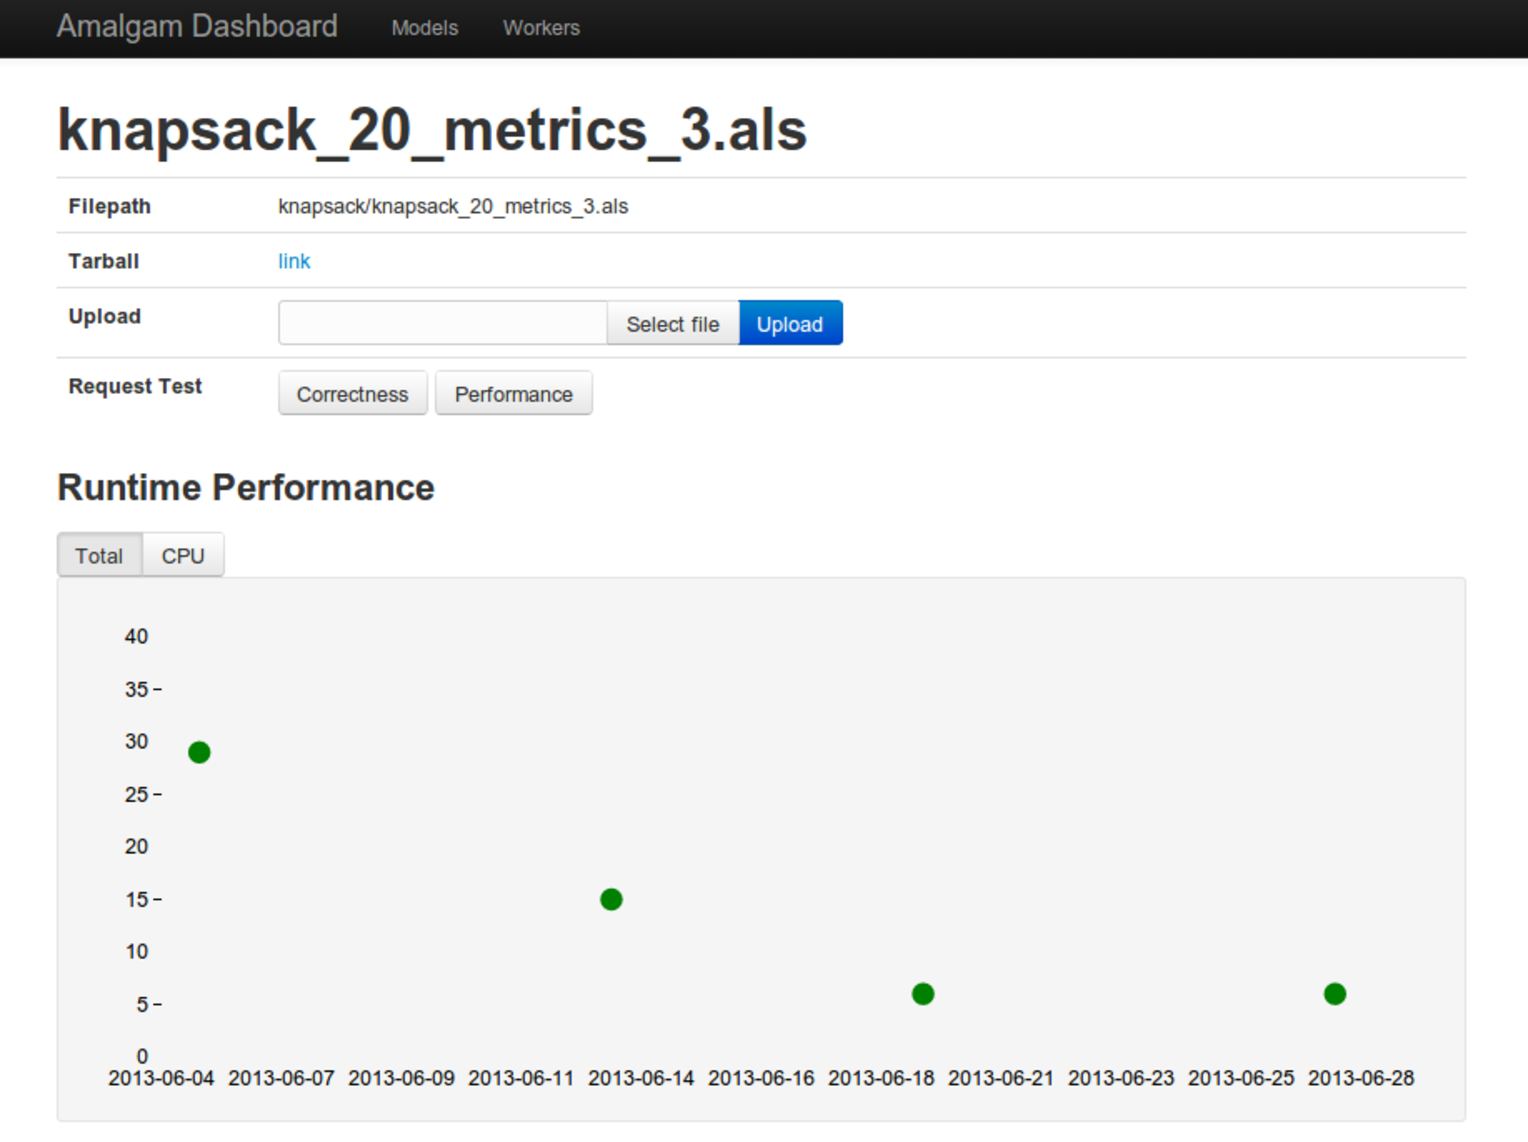
\includegraphics[width=\textwidth]{images/model_view}
\end{figure}

\subsubsection{Workers}
The worker page shows the list of all the workers that are currently online and their status. The view of the worker page for our dashboard is show in appendix \ref{app:dashboard} figure \ref{fig:dashboard_workers}. As can be seen in the figure our testing infrastructure currently has 10 active workers running performance tests. The green rows shows workers that are online and the red rows shows the servers that are unreachable. This usually means either that the server is turned off or it is unreachable through the network.

The motivation for creating this page is to allow us to see which workers are running and which workers are not so that in case there are failures, we can immediately investigate the issue to ensure that our performance tests are not delayed. Performance delays due to system failure do not skew our perormance results because whenver there is system failure the interrupted test is re-run and the computation time is recorded. As can be visible from the page, currently 3 of our servers are in an inactive state and 7 of the server are active/online.

\subsection{Job Queue and Workers: CS servers}
Currently we are using 7 of the CS servers to run our tests 1 of which is inactive. We also have access to 3 servers which are running Core i7 processors in the WatForm laboratory under the CS faculty. Access to these server has been made available to us through our project consultant Derek Rayside. The three servers in WatForm are called ``digby'' and ``daedulus-ubuntu''.

The job scheduling queue is maintained by the dashboard to schedule runs for the workers whenever there is a manual test request or a new build has been created by the continuous integration system.

%%%%%%%%%%%%%%%%%%%%%%%%%%%%%%%%%%%%%%%%%%%%%%%%%%%%%%%%%%%%%%%%%%%%%%%
\section{Pre-implementation and Testing Infrastructure}\label{sec:implementation}
Since the start of our project towards the end of Fall 2012, we have made satisfactory progress on our project. The project has 2 basic activities in the pre-developement phase. Much of it done during our co-op term in Winter 2014 and a significant portion of it has been done this term in the last two months.

\subsection{Creating Test Models}
Our first task for the project was to take the semantic model description and write Alloy models to describe these semantic models that can be used by Moolloy to find solutions. The exercise involved us having to learn Alloy and build our skills in writing relational models. Much of our work during the Fall term was spent on adapting this learning curve necessary for writing dependable relational models for multi-objective problem. Before the beginning of our co-op terms we divided up the model sets among the members so that we could work on them concurrently.

We had six categories of problems. For more details on the problems please refer to \cite{ref:Rayside09}:

\begin{enumerate}
\item Aerospace problems from NASA
\item Knapsack problem of variying complexity
\item N-Queens problems of varying complexity
\item N-Rooks problems of varying complexity
\item Software Product Line Problems
\item Civil Engineering problems from Dr.\ Patrick Reed, University of Waterloo.
\end{enumerate}

Between all the categories we had roughly 250 different problem sets. With continuous collaboration during the co-op term, we were able to convert 212 different working models for our project. The toy model sets in the category of \emph{Knapsack, N-Queens and N-Rooks} were some of the easier categories to convert. While some of the real life problems such as \emph{Aerospace, SPL and Civil Engineering} problems are far more difficult because of the engineering challenge behind being able to encode all the necessary constraints of the physical model into relational logic. Most of the incomplete models were in the category of the civil engineering problems due to the unclear definitions and technical deficiencies on our part in understanding the advanced civil engineering concepts and grasping their semantics. A sample of one of the simpler knapsack problems is presented in appendix \ref{app:knapsack}

\subsection{Testing Dashboard}
Much time was also spent during the co-op on setting up the testing dashboard as described in the previous sections. At a certain stage when we had a sizeable collection of models we started doing this concurrently to test the models that we were creating for correctness. It was an incremental design process and we added elements to it as we felt was needed. Initially we started with the seven CS workers and currently we have 10. Our most recent addition to the testing dashboard has been the distinction between the CPU run-time and the overall run time distinction or the models as well the graphical representation of the models in the models window which we finished within the second week of the Spring '13 term.

\subsection{Refactoring and Unit Tests for Existing Code} \label{sec:refactor}
Before working on implementing the actual features we realized we needed to refactor the current code base of Moolloy to help us in the implementation process.

One of the major code refactoring we made was refactoring the \emph{Guided Improvement Algorithm} from its original location in the codebase of \emph{Alloy} to be in the code base for \emph{Kodkod}. We thought this would be a more appropriate location for the implementation of the Guided Improvement Algorithm because Kodkod is the abstraction that actually calls the SAT solver by converting the model to logic formulae. Therefore moving the algorithm to a lower abstraction allowed us to implement some Formula optimization and compiler optimizations on the relational logic models. These changes were basically about integrating Multi-objective optimization solving functionalities in Kodkod and it required some engineering study regarding relational logic solver optimizations. As a result of this refactoring process we already saw improvements in many of our models in the order of 10 to 20\%.

During the refactoring process we also started writing unit tests for the specific steps of the algorithm and different modules to make sure we were not breaking any of the existing code and introducing regressions during the refactoring process. The unit test API used for these purposes was JUnit \cite{ref:junit} since the code base for Moolloy is in Java.

This process took us about 2 to 3 weeks this term to complete and much of the time was spent in debugging the refactoring steps and implementing the integration features to the Kodkod codebase to compute solutions for multi-objective optimization problems.

\section{Implementing Optimization Features}
This term we are currently working on implementing two improvement features to the \emph{GIA} codebase. The first feature are woring on currently is implementing incremental solving capabilities for Kodkod. The second feature we will be working on is implementing multi-threaded concurrent solving capabilities to Kodkod for computing solutions for multi-objective optimization problems. The implementation approach and some of the challenges behind the approaches are described in the following subsections.

\subsection{Incremental Solving Capabilities}
When Kodkod makes calls to the SAT solver to get solutions for different objectives, it get solutions by incrementally pushing constraints to the models to get optimal solution for higher constraints. Basically, it tries to get the most optimal solution that fits as many of the objectives as possible. When it can't find any more solutions that can satisfy a set of objective constraints it takes a step back by removing a constraint and retry solving the problem with a different set of constraints.

The problem with the current implementation of Kodkod is that it does not do incremental solving, which means that each time kodkod needs to push constraints to a model it has to re-calculate all the solutions it computed for the more relaxed model and build from that. Incremental solving capabilities allow Kodkod to store partial instance of metric points and for tighter constraints build from the existing solution set to compute for satisfiable solutions within the tighter constraints without having to reconstruct the entire solution space for deeper metric points in the search tree.

After implementation of the incremental solver for Kodkod for some models we saw drastic performance improvements sometimes in the order of 200\% (4 times). One such model is the knapsack model in figure \ref{fig:modelview}. However for some of the larger models we surprisingly saw a decrease in performance  which was unexpected. We are currently in the process of investigating the reason for this and resolving the regression. The current hypothesis is that because of the incremental solving technique, the servers are reaching a memory bottleneck because for higher order models the solver needs to keep track of all the partial instances for the solution space, resulting in context switching for all solver calls for deeper pareto points resulting in slower computation times. Therefore we are looking into running our program through a memory profiling tool to detect the source of the memory leakage.

\subsection{Concurrency}
One of the subgroups of our team is looking into the implementation of concurrency to solve multi-objective optimization problems. The basic idea is that when we want to build on a certain solution by incrementing constraints, we should be able to explore different computation spaces concurrently without compromising the integrity of other branches.

We are currently investigating the use of Java concurrency and synchronization packages to implement concurrency for the algorithm implementation. One of the major challenges of implementing concurrency in this case is differentiating duplicate solutions across threads. This means that if two threads are doing their computations completely independently it is very possible that two threads might end up finding the same solution from the SAT solver. The problem of differentiating between similar points become even more difficult as the problem scales to multiple dimensions due multiple objectives.

We have explored multiple possible ways of solving this problems. The basic idea we are follwing to solve this problem is that for concurrent solving we want find a smart way of partitioning SAT solver computations so that two separate threads would not be finding the same metric point. We are still in the stage where we want to implement the multiple ideas of solving the problem and test the results for correctness.

\subsection{Using an SMT solver instead of SAT solver}
According to some preliminary research by a grad student working on relavant areas, SMT solvers in this domain are much more efficient at finding solutions to multi-objective problem defined by numeric metrics definitions. The reason for this is because SMT solvers can actually do numeric computations as well as relational logic solving which make the computation much faster because SAT solvers do not have a concept of arithmetic. Because of this limitation of SAT, Kodkod has to decompose arithmetic operations into partial instances using bit blasting techniques to encode arithmetic operations into boolean circuits \cite{ref:bitblasting}. Using SMT solver instead of SAT makes the computations much faster during the metric comparisons and therefore this makes the computations much faster. Implementing the Guided Improvement Algorithm using SMT solvers would be challenging because we would have to explore ways of expressing the formulae to pass to the solver in the best possible way for optimality.

%%%%%%%%%%%%%%%%%%%%%%%%%%%%%%%%%%%%%%%%%%%%%%%%%%%%%%%%%%%%%%%%%%%%%%
\section{Progress Assessment}\label{sec:progress}
Throughout the lifetime of our project we usually made short-term goals and long-terms goal. This section does an assessment of the status of our long term and short term goals and also our goals in the future.

\begin{figure}[H]
	\caption{Long Term Planning} \label{fig:longterm}
	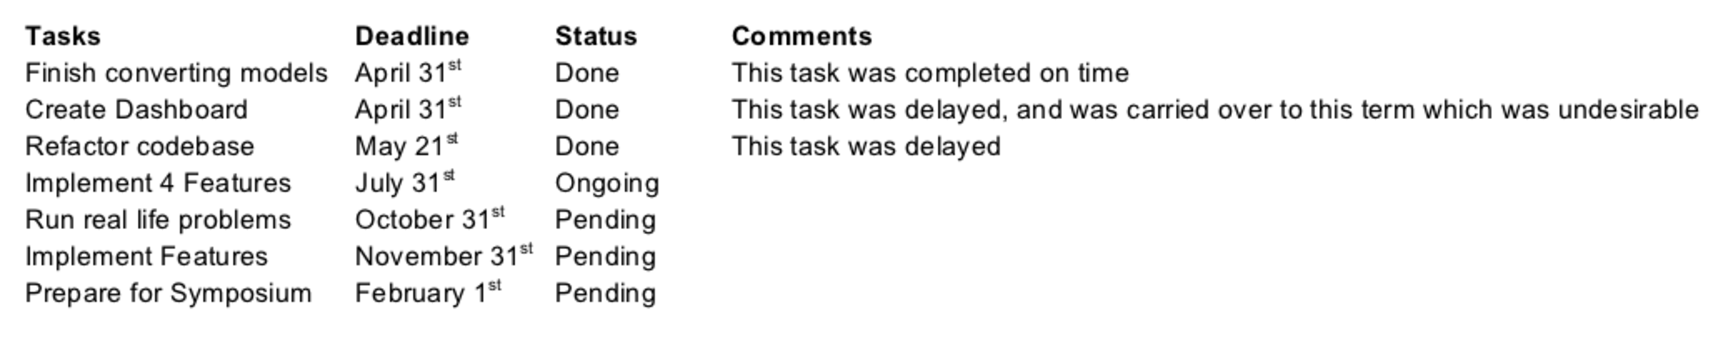
\includegraphics[width=\textwidth]{planning/longterm}
\end{figure}

Figure \ref{fig:longterm} refers to the planning chart for our activities on the long term. So far all our activities related to setting up the project is completed which includes writing the test models, creating the testing dashboard and refactoring the code base to support our features. Among them the refactoring process and creating the dashboard took longer than expected. For the dashboard we kept on adding features that we thought were necessary as we tested the models so the delay was justified although unexpected. For the refactoring task, it proved to be a more challenging task than expected because we have to make significant changes to the code base of Kodkod to reimplement the Guided Improvement Algorithm in it. Also figuring our some of the formula optimization, as talked about in section \ref{sec:refactor}, took a little longer because we had to hand calculations in boolean logic and test the results.

We do feel that we are on track for finishing the implementation of the 4 features that we want to implement within this term. This is seen better detail in figure \ref{fig:shortterm} where the short term objectives for the current terms are shown. We have partially implemented two of the features and we have started working on the concurrency feature, which means that in the next 4 weeks we need to finish the current features, which are progressing according to schedule, and finish the SMT solver feature, and that does seems like a feasible plan at the moment. 

We have also decided to break up the tasks in pairs. This is because most of the features require a certain level of research and some paper-and-pencil exercises. From past experiences we have noticed that for such intensive activities it is easier to work in pairs because it helps produce better quality and avoid bugs in the feature.

\begin{figure}[H]
	\caption{Short term planning for this term } \label{fig:shortterm}
	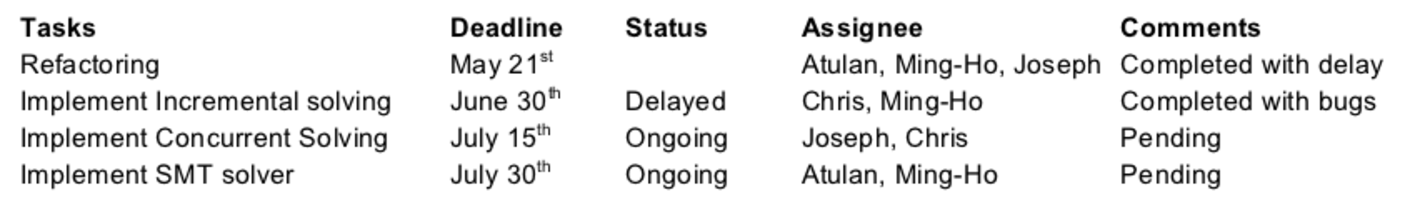
\includegraphics[width=\textwidth]{planning/shortterm}
\end{figure}

Looking beyond this term, over the co-op term we want to finish implementing further features we can think of that might improve performance and most importantly check to see that the improved algorithm can successfully run more complicated real-life problems such as the \emph{Aerospace and Civil Engineering} problems that take much longer to run or are unsolvable using the current version of the algorithm. 

One of possible improvement we may need to make to the algorithm is explore how we can also make it more memory efficient, because for larger problems this might prove to be a bottle neck. This might require exploring heuristics to explicitly call the garbage collector to free up space for unnecessary immutable objects in the heap. It is in our list of tentative features to implement in the future.

\pagebreak

% Appendices
\appendix

%%%%%%%%%%%%%%%%%%%%%%%%%%%%%%%%%%%%%%%%%%%%%%%%%%%%%%%%%%%%%%%%%%%%%%
\section{Guided Improvement Algorithm}\label{app:impl}

This appendix outlines, at a high-level, how the \textit{guided
improvement algorithm} works. Rayside et al.~\cite{ref:Rayside09}
provide a more formal and detailed description in their paper.

First, Moolloy finds a solution that satisfies the constraints. Once
this solution is found, Moolloy finds a new solution that dominates the
previous one. Moolloy continues this process of finding new solutions
until no other dominating solution can be found---this last solution is
on the Pareto front, by definition.

Moolloy continues this process with new starting solutions (that are
not dominated by any previously discovered solution) until all
solutions on the Pareto front are found.

Thus, Moolloy makes a large number of calls to the underlying SAT
solver. These are extremely expensive calls, so the goal for optimizing
Moolloy is to reduce the number of calls to the SAT solver.

%%%%%%%%%%%%%%%%%%%%%%%%%%%%%%%%%%%%%%%%%%%%%%%%%%%%%%%%%%%%%%%%%%%%%%%%
\pagebreak
\section{Alloy Model: Knapsack, 10 metrics, 2 objectives}\label{app:knapsack}
\begin{verbatim}
  open util/integer
  pred show {}
  
  abstract sig Item {
    weight : one Int,    
      metric0 : one Int ,    
      metric1 : one Int     
  }

  abstract sig Knapsack {
    items : set Item,
    max_weight : one Int,
    current_weight : one Int,    
      metric0 : one Int ,    
      metric1 : one Int 
  }

  // Metric of the knapsack is sum of item metrics
  
    fact { all k : Knapsack | k.metric0 = (sum i : k.items | i.metric0)}
    fact { all k : Knapsack | k.metric1 = (sum i : k.items | i.metric1)}
  
  // Weight of knapsack is sum of item weights
  fact { all k : Knapsack | k.current_weight = (sum i : k.items | i.weight)}
  
  // Weight of knapsack must be less than the max weight
  fact { all k : Knapsack | k.current_weight <= k.max_weight }

  // Define concrete items
  
    one sig Item0 extends Item {} {
      weight = 3      
        metric0 = 4       
        metric1 = 6       
    }
  
    one sig Item1 extends Item {} {
      weight = 0      
        metric0 = 2       
        metric1 = 2       
    }
  
    one sig Item2 extends Item {} {
      weight = 1      
        metric0 = 9       
        metric1 = 6       
    }
  
    one sig Item3 extends Item {} {
      weight = 0      
        metric0 = 2       
        metric1 = 8       
    }
  
    one sig Item4 extends Item {} {
      weight = 5      
        metric0 = 9       
        metric1 = 5       
    }
  
    one sig Item5 extends Item {} {
      weight = 7      
        metric0 = 7       
        metric1 = 10       
    }
  
    one sig Item6 extends Item {} {
      weight = 2      
        metric0 = 1       
        metric1 = 8      
    }
  
    one sig Item7 extends Item {} {
      weight = 7      
        metric0 = 10       
        metric1 = 7       
    }
  
    one sig Item8 extends Item {} {
      weight = 0      
        metric0 = 9       
        metric1 = 5      
    }

    one sig Item9 extends Item {} {
      weight = 3      
        metric0 = 7       
        metric1 = 2  
    }

  // Define concrete knapsack
  one sig ConcreteKnapsack extends Knapsack {} {
    max_weight = 100
  }

  inst KnapsackProblem {
    8 Int
  }

  objectives o_global {    
      maximize ConcreteKnapsack.metric0 ,
      maximize ConcreteKnapsack.metric1     
  }

  run show for KnapsackProblem optimize o_global

\end{verbatim}
\pagebreak
\section{Dashboard Views}\label{app:dashboard}
\begin{figure}[H] 
	\caption{Dashboard:Homepage}\label{fig:dashboard_home}
	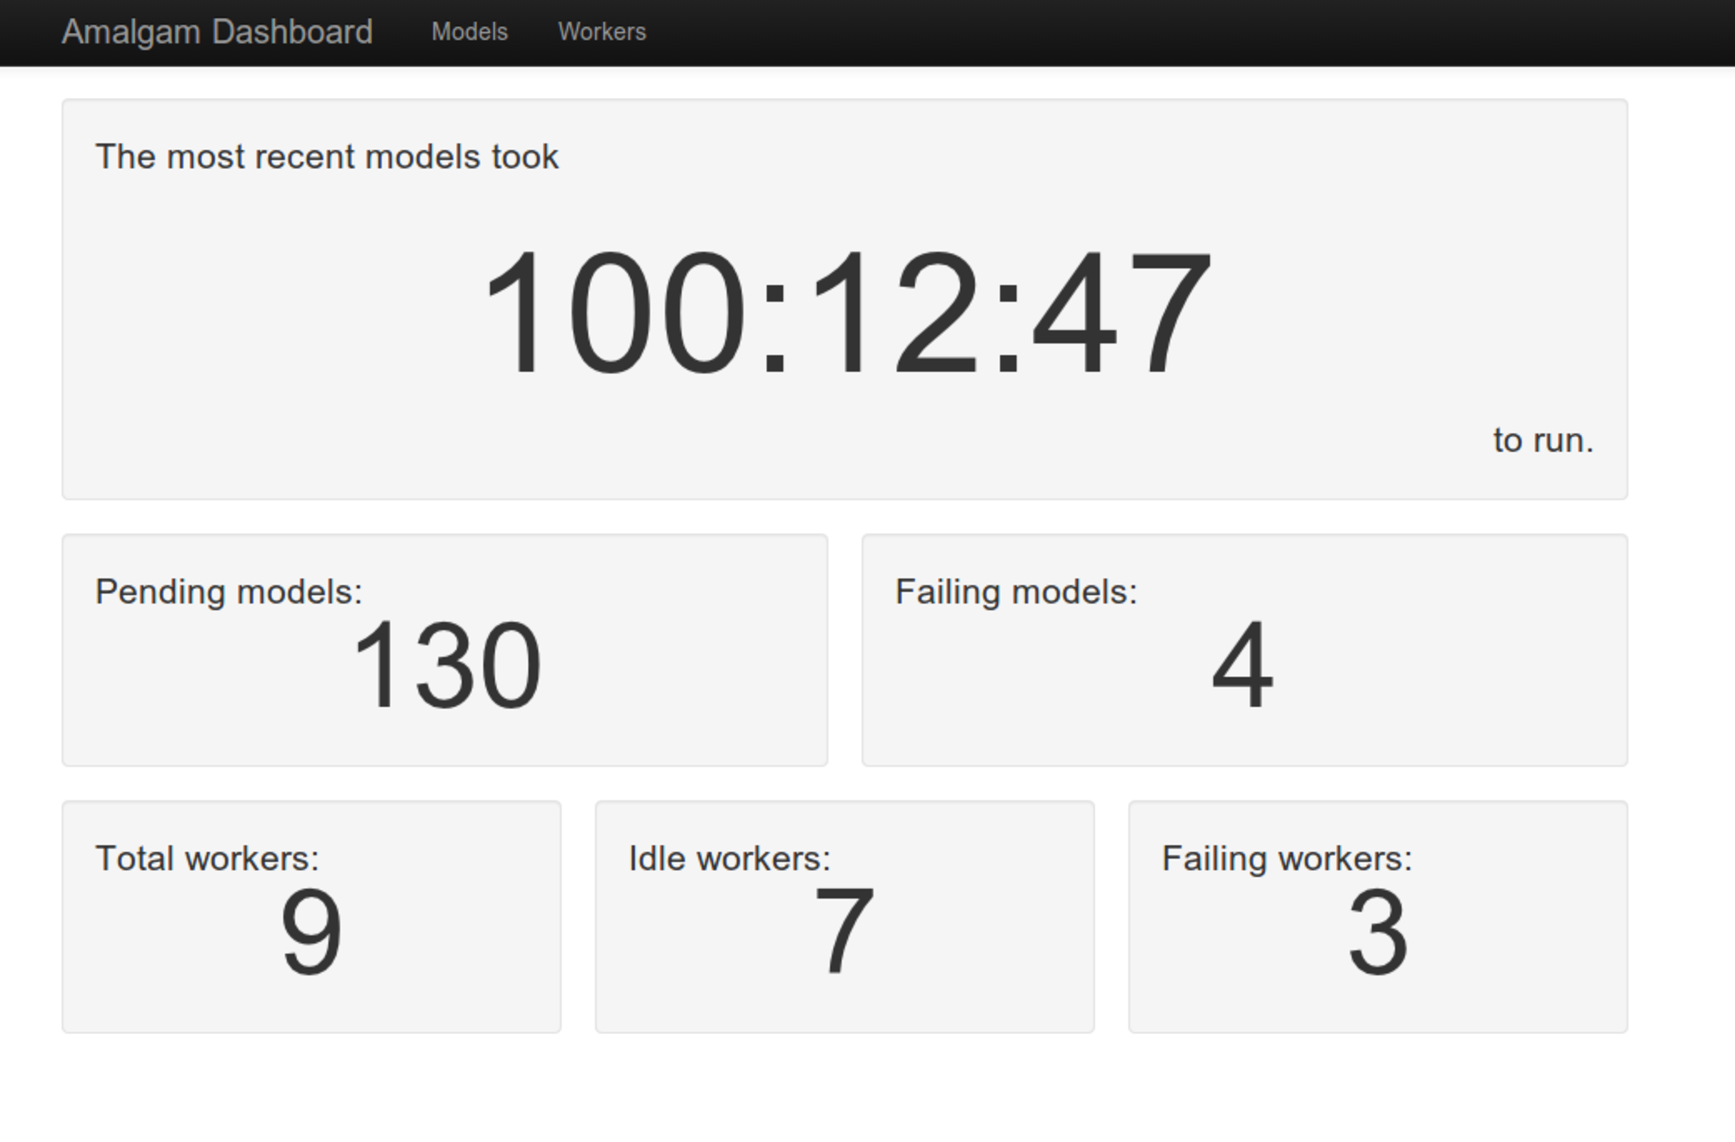
\includegraphics[width=\textwidth]{images/dashboard_home}
\end{figure}

\begin{figure}[H] 
	\caption{Dashboard:Models}\label{fig:dashboard_models}
	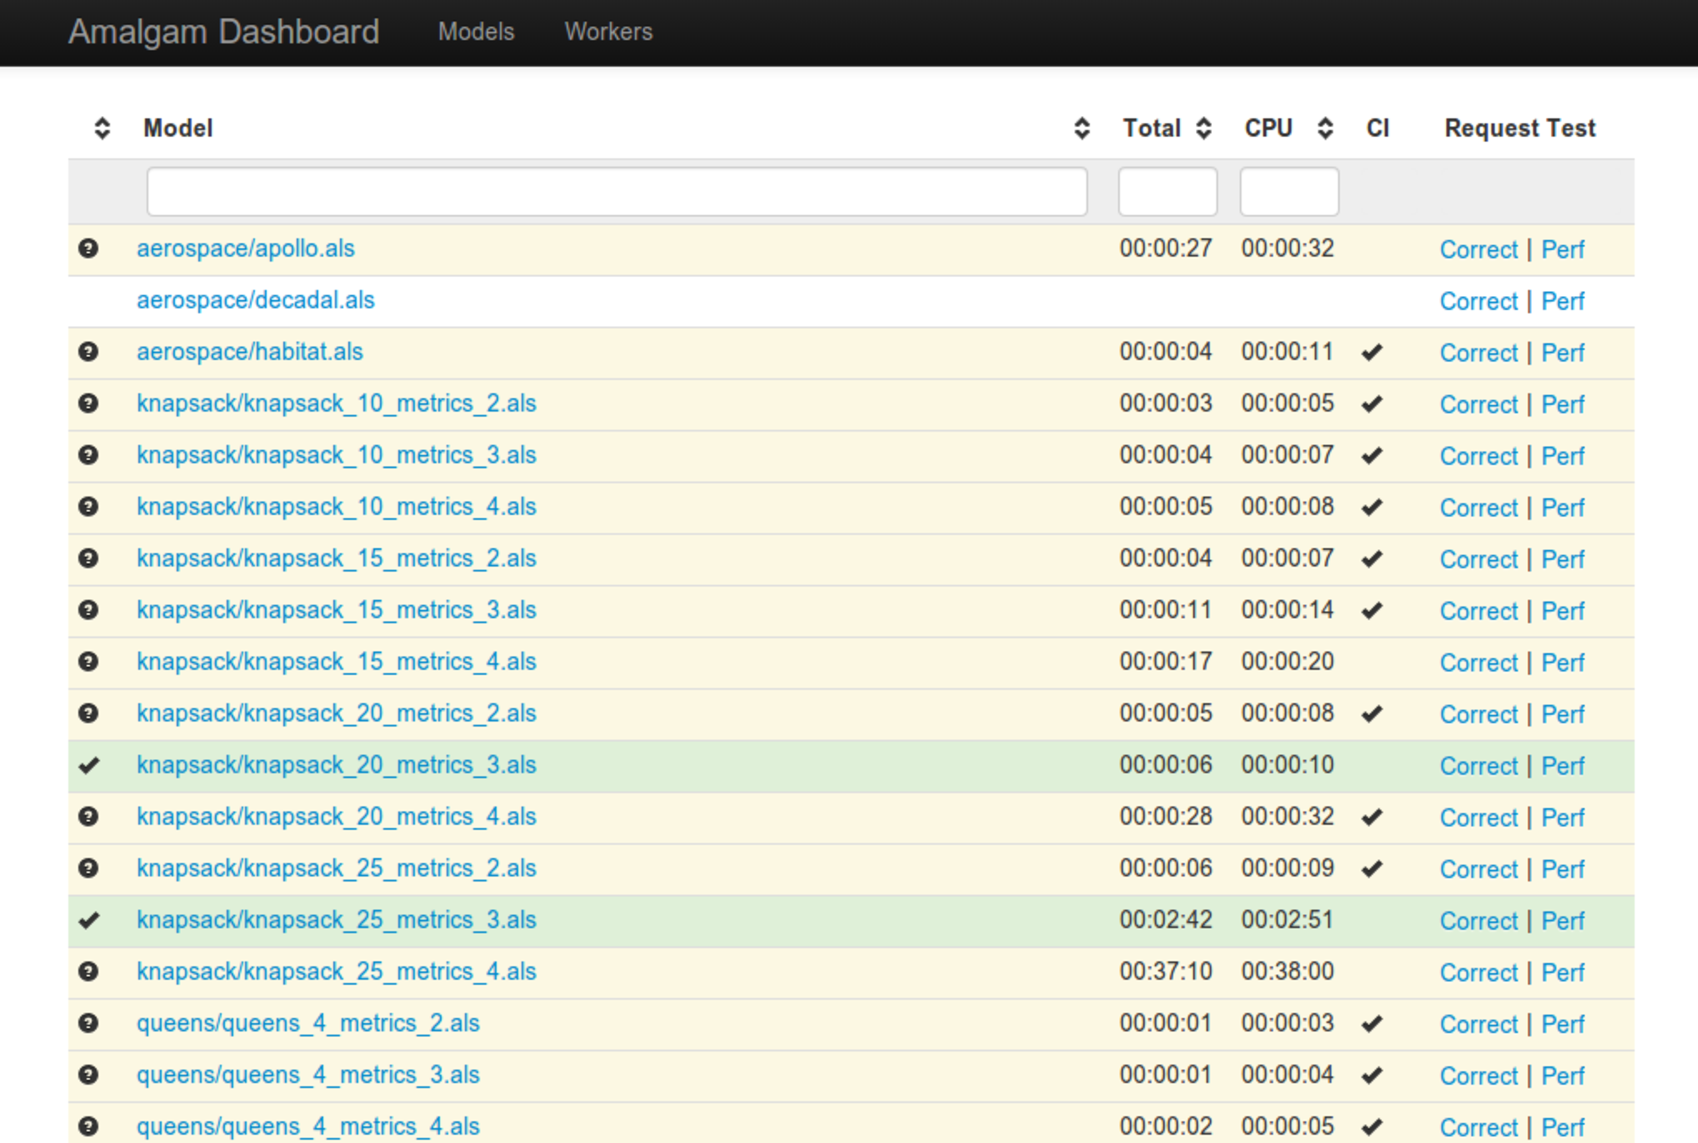
\includegraphics[width=\textwidth]{images/dashboard_models}
\end{figure}

\begin{figure}[H] 
	\caption{Dashboard:Workers}\label{fig:dashboard_workers}
	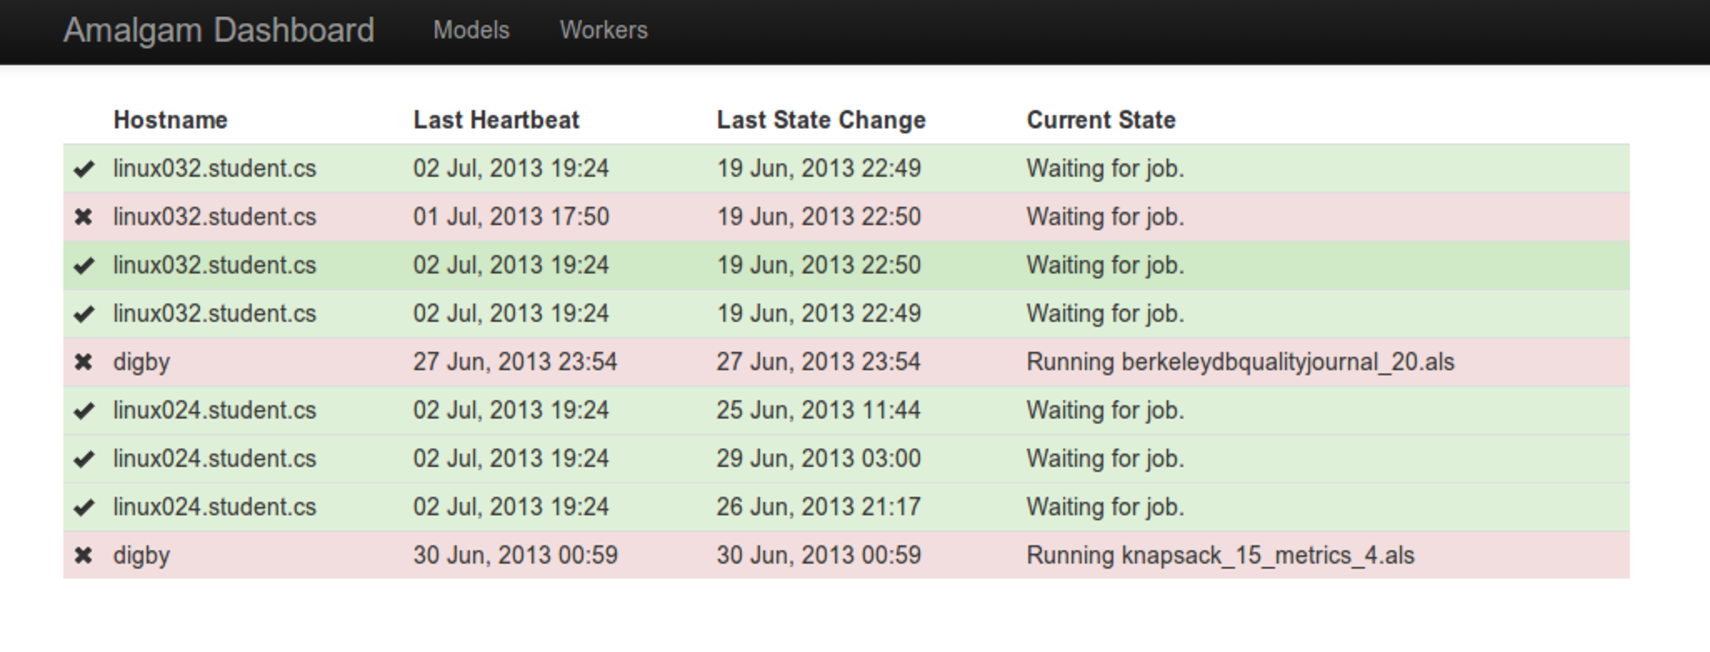
\includegraphics[width=\textwidth]{images/dashboard_workers}
\end{figure}

\pagebreak

\bibliographystyle{IEEEtran}
\bibliography{detail}


\end{document}
